\section{Simulation}
\subsection{Polymermodell}

\begin{frame}
       \begin{tabular}{cl}
         \begin{tabular}{c}
           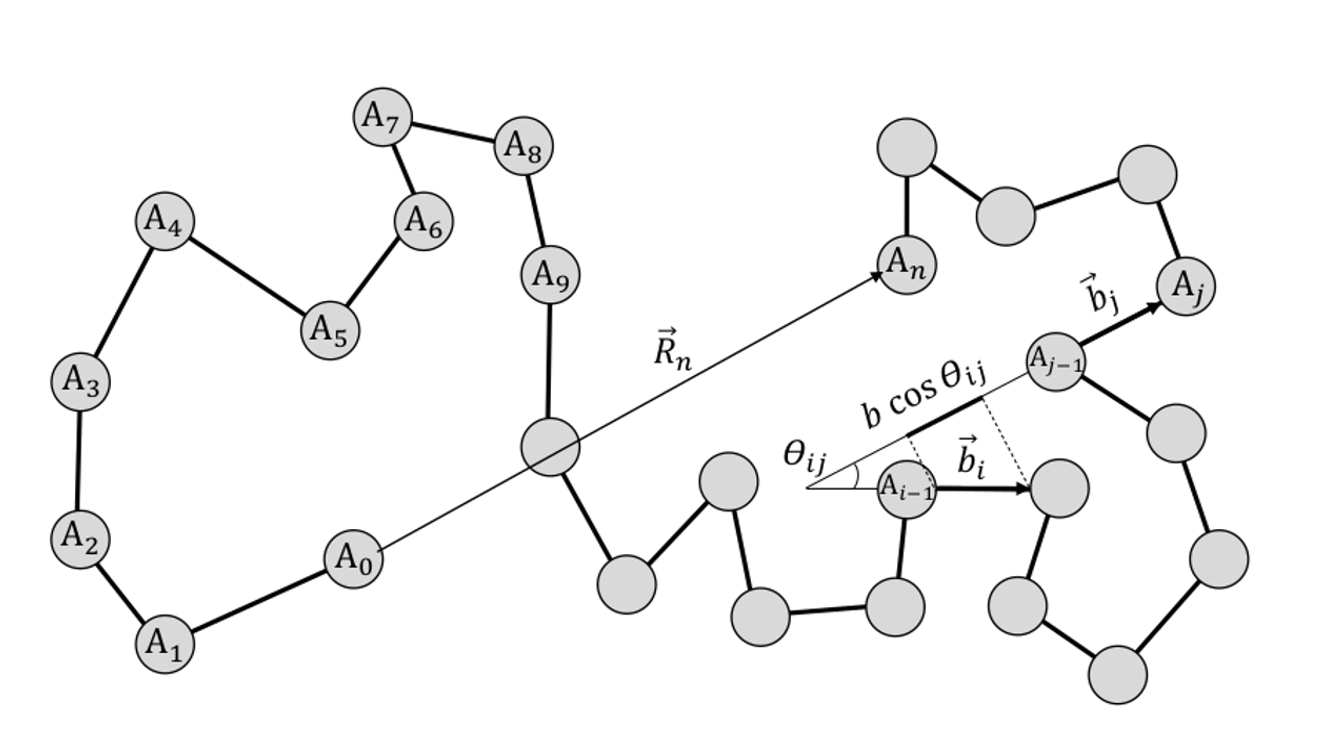
\includegraphics[width=0.5\textwidth]{Plots/rubinstein.png}
           \end{tabular}
           & \begin{tabular}{l}
             \parbox{0.5\linewidth}{
             \begin{itemize}
               \setlength\itemsep{1em}
               \item Monomere bestehen aus \textit{beads}\\ und \textit{bonds} \\
               \item N Monomere \\(Polymerisationsgrad)
               \item Bondvektoren $\vec{b}_i$ mit Länge $b$ \\
             \end{itemize}

             }
             \end{tabular}  \\
         \end{tabular}
         \begin{tiny}Quelle: Rubinstein, Michael and Colby, Ralph H. - Polymer Physics\\
         \end{tiny}
         \begin{itemize}
           \item $\Theta_{ij}$ ist Winkel zwischen $\vec{b}_i$ und $\vec{b}_j$ \\
           \item End-zu-End-Abstand $\vec{R}=\sum_{i=0}^{N-1} \vec{b}_i$
         \end{itemize}
\end{frame}

%\begin{frame}
%  \frametitle{wichtige Messgrößen}
%  \begin{block}{Definitionen}
%     \begin{itemize}
%       \item $\langle O \rangle = \frac{1}{Z} \sum_{i} O \text{e}^{-\beta E_i}$
%       \item $Z = \sum_i \text{e}^{-\beta E_i}$
%       \item $\langle R^2 \rangle = b^2 \sum_{i=0}^{N-1} \sum_{j=0}^{N-1} \langle \text{cos} \, \Theta_{ij} \rangle$
%       \item $\vec{t}_i = \frac{\vec{b}_i}{b}$
%       \item $\vec{t}_i \cdot \vec{t}_j = \text{cos} \, \Theta_{ij}  = \text{exp}{\left(- \frac{\lvert i - j \rvert}{ L_{\mathrm{p} }} \right)} $
%     \end{itemize}
%  \end{block}
%\end{frame}
\begin{frame}
   \frametitle{Wormlike-Chain (WLC)}
   \begin{block}{Definition über die Biegeenergie}
     \begin{itemize}
       \item $\vec{t}_i = \frac{\vec{b}_i}{b}$
       \item $\kappa = E \cdot I \sim E \cdot a^4$
       \item $E_{\text{bond}} = \frac{\kappa}{b} (1 - \text{cos}\,\Theta_{i-1,i})$
       \item $E_{\mathrm{Biege}}^{\mathrm{Ges}} = \frac{\kappa}{2b}\,\sum_{i=1}^{N-1} \left( \vec{t}_{i-1} - \vec{t}_{i}  \right)^2$
       \item $ \langle \vec{t}_i \cdot \vec{t}_j \rangle = \langle \text{cos} \, \Theta_{ij} \rangle  = \text{exp}{\left(- \frac{\lvert i - j \rvert}{ L_{\mathrm{p} }} \right)} $
     \end{itemize}
   \end{block}
   \begin{block}{Persistenzlänge der WLC}
     \begin{itemize}
       \item $L_{\mathrm{p}} = -\frac{b}{\coth \frac{\kappa}{b\,\mathrm{k_B\,T}} - \frac{b}{\kappa}\,\mathrm{k_B} \, T }$
     \end{itemize}
  \end{block}
\end{frame}

\begin{frame}
  \frametitle{Klassifizierung nach Flexibilität}
  \begin{figure}
    \centering
    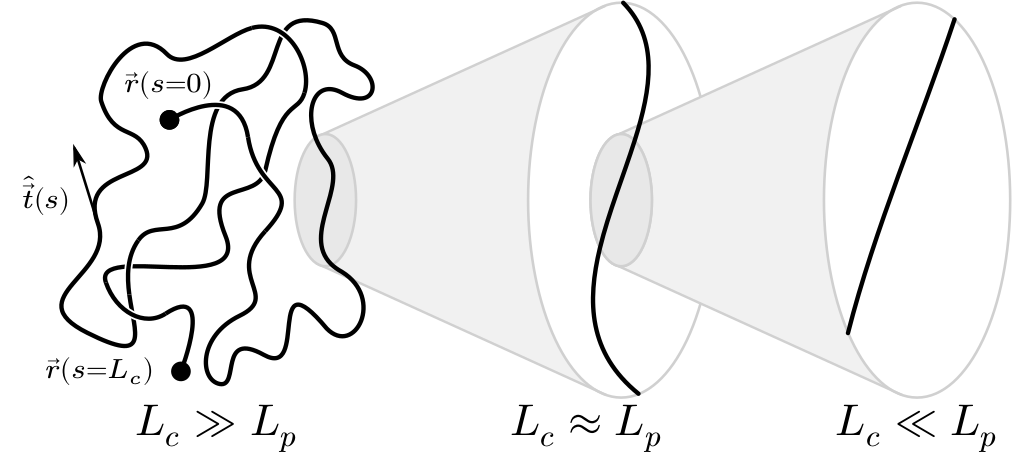
\includegraphics[width=\textwidth]{Plots/regime.png}
    \caption{Quelle: Dissertation Tobias Kampmann}
    \label{fig:regime}
  \end{figure}
\end{frame}

\subsection{Monte-Carlo Simulation}

\begin{frame}
  \frametitle{Markow-Sampling}
  \begin{itemize}
    \item Berechnung von Erwartungswerten, mittels Zufallsprozessen
    \item Sampling vereinfacht Erwartungswert zu $\langle O \rangle = \frac{1}{n} \sum_{i=0}^n O(i)$
    \item Dafür zwei Bedingungen: \\
          \begin{enumerate}
            \item Detailliertes Gleichgewicht
            \item Ergodizität
          \end{enumerate}
  \end{itemize}
  \begin{block}{Detailliertes Gleichgewicht}
    \begin{itemize}
      \item $\frac{m_{ij}}{m_{ji}} = \frac{p_j}{p_i}$
    \end{itemize}
  \end{block}
\end{frame}

\begin{frame}
  \frametitle{Metropolis Algorithmus}
  \begin{itemize}
    \item Vorschlagsmoves mit Vorschlagswahrscheinlichkeit $V_{ij}$
    und Akzeptanzwahrscheinlichkeit $A_{ij}$
    \item $m_{ij} = V_{ij}A_{ij}$
  \end{itemize}
  \begin{block}{Metropolis-Filter}
    \begin{itemize}
      \item $A_{ij} = \text{min}( 1, \frac{p_i}{p_j})$
      \item $V_{ij} = V_{ji}$
    \end{itemize}
  \end{block}
  \begin{itemize}
    \item $p_i \propto \text{exp}(-\beta E_i)$
  \end{itemize}
\end{frame}

\begin{frame}
  \frametitle{Monte-Carlo-Moves}
  \begin{enumerate}
    \item Wähle zufälligen Bead
    \item Drehe zugehörigen Bondvektor, um $\Delta\Theta$
    \item $\Delta E = E_{\text{alt}}-E_{\text{neu}}$
    \item Fallunterscheidung:\\
         \setbeamertemplate{enumerate items}[square]
         \begin{enumerate}
           \item $\Delta E \geq 0$: akzeptiere Vorschlag
           \item $\Delta E < 0$: akzeptiere mit Wahrscheinlichkeit
                 $\text{exp}(\beta \Delta E)$
         \end{enumerate}
  \end{enumerate}
\end{frame}

\begin{frame}
\begin{minipage}[t]{0.5\textwidth}
\includegraphics[width=\textwidth]{Plots/Energie.pdf}
\end{minipage}%
\hfill%
\begin{minipage}{0.5\textwidth}
\begin{itemize}
  \item Parameter $N=100$, $b=1$, $\kappa=100$, $\beta = 1$
  \item zufällige Anfangskonfiguration
  \item Äquilibrierungszeit von ca. $10^3$ Durchläufen
  \item Äquipartitionstheorem: $\langle E \rangle = 1\,\text{k}_{\text{B}}T$
        pro Bond
\end{itemize} \vspace{2.5cm}
\end{minipage}

\end{frame}


\begin{frame}
  \frametitle{Tangentenkorrelationen}
  \begin{itemize}
    \item $L_{\mathrm{p}} = -\frac{b}{\coth \frac{\kappa}{b\,\mathrm{k_B\,T}} - \frac{b}{\kappa}\,\mathrm{k_B} \, T } \approx 99.5 $ \\
    \item $\langle \vec{t}_i \cdot \vec{t}_{i+j} \rangle = \sum_{i=0}^{N-1-j} \vec{t}_i \cdot \vec{t}_{i+j}$
  \end{itemize}
  \begin{figure}
    \centering
    \includegraphics[width=0.6\textwidth]{Plots/korr13.pdf}
    \label{fig:tangkorr}
  \end{figure}
\end{frame}

\begin{frame}
  \frametitle{Erzeugung von Messwerten}
  \begin{minipage}{0.4\textwidth}
  \begin{itemize}
    \item künstliches Neuronales Netz soll aus Polymerkonfiguration
          dessen Biegesteifigkeit bestimmen
    \item $N=100$, $b=1$, $\beta = 1$
    \item $10 \leq \kappa \leq 20$
    \item Momentaufnahme: Winkel $\Theta_{i-1,i}$, $\kappa$
  \end{itemize}
  \end{minipage}%
  \hfill%
  \begin{minipage}{0.4\textwidth}
  \includegraphics[width=\textwidth]{Plots/polymer1.pdf}
  \end{minipage}\\
  \begin{minipage}{0.4\textwidth}
    \begin{figure}
     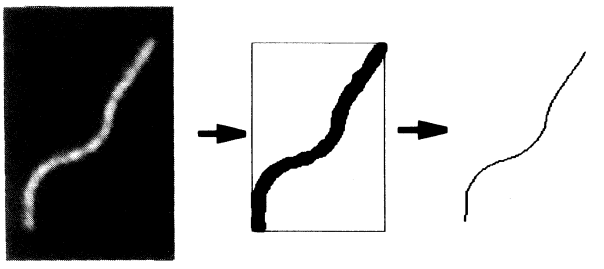
\includegraphics[width=\textwidth]{Plots/pixel-reduction.png}
     \caption{\url{https://link.aps.org/doi/10.1103/PhysRevE.48.R1642}}
    \end{figure}
  \end{minipage}%
  \hfill%
  \begin{minipage}{0.4\textwidth}
    \begin{figure}
    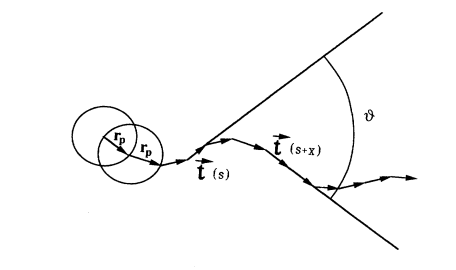
\includegraphics[width=\textwidth]{Plots/fluorescene-winkel.png}
    \end{figure}
  \end{minipage}
\end{frame}

\begin{frame}
  \frametitle{Beispielkonfigurationen}
  \begin{figure}
    \centering
    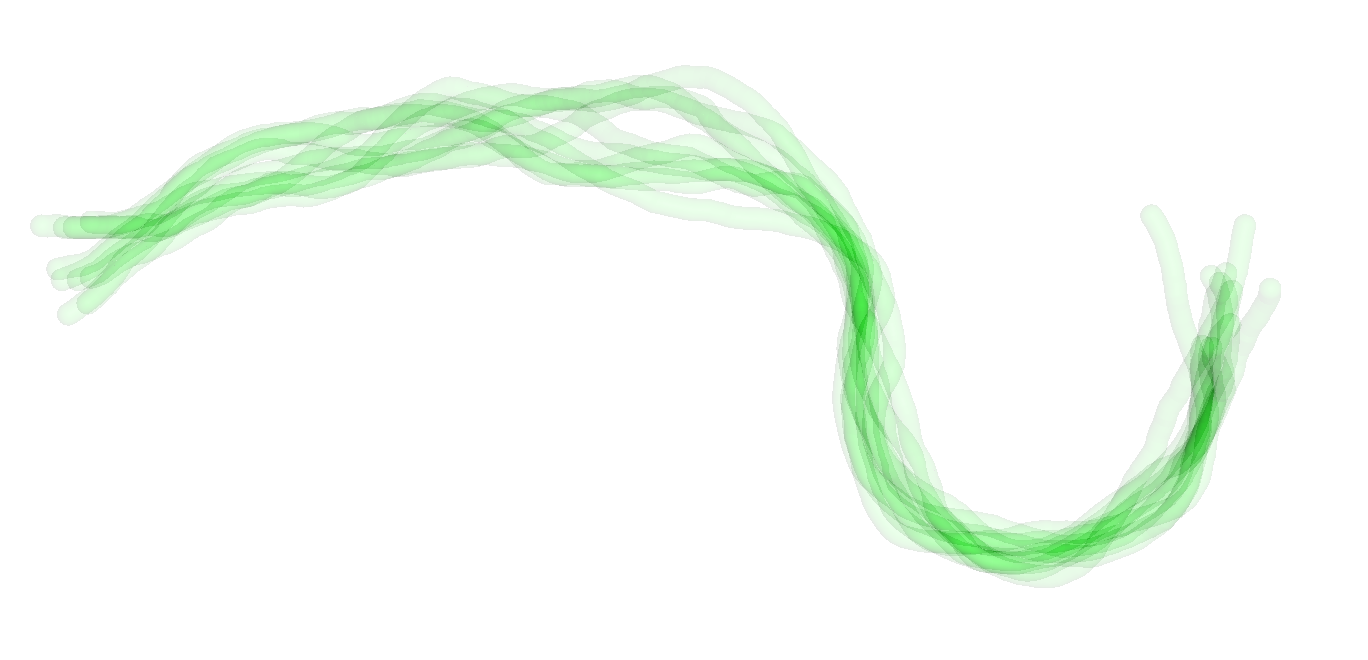
\includegraphics[width=\textwidth]{Plots/blurred33.png}
    \label{fig:bsp}
  \end{figure}
\end{frame}
